\documentclass[tikz,border=10pt]{standalone}
\usepackage{fontspec}
\setmainfont{Latin Modern Roman}
\usetikzlibrary{arrows.meta}
\begin{document}
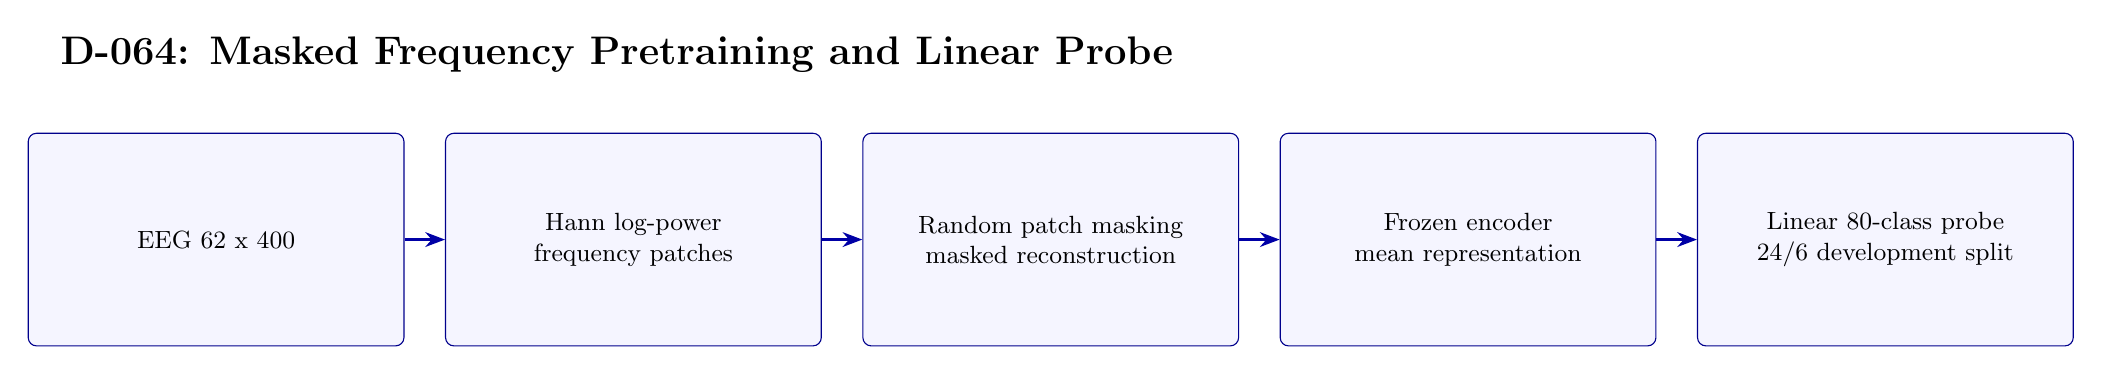
\begin{tikzpicture}[block/.style={draw=blue!55!black,fill=blue!4,rounded corners=3pt,align=center,text width=4.35cm,minimum height=2.7cm,inner sep=6pt,font=\small},arrow/.style={-{Stealth[length=2.5mm]},line width=1pt,draw=blue!65!black}]
\node[font=\Large\bfseries,anchor=south west] at (-2.1,2.0) {D-064: Masked Frequency Pretraining and Linear Probe};
\node[block] (n0) at (0.0,0) {EEG 62 x 400};
\node[block] (n1) at (5.3,0) {Hann log-power\\frequency patches};
\node[block] (n2) at (10.6,0) {Random patch masking\\masked reconstruction};
\node[block] (n3) at (15.899999999999999,0) {Frozen encoder\\mean representation};
\node[block] (n4) at (21.2,0) {Linear 80-class probe\\24/6 development split};
\draw[arrow] (n0) -- (n1);
\draw[arrow] (n1) -- (n2);
\draw[arrow] (n2) -- (n3);
\draw[arrow] (n3) -- (n4);
\end{tikzpicture}
\end{document}
